\documentclass[aspectratio=169]{beamer}
%
% Choose how your presentation looks.
%
% For more themes, color themes and font themes, see:
% http://deic.uab.es/~iblanes/beamer_gallery/index_by_theme.html
%
\mode<presentation>
{
  \usetheme{default}      % or try Darmstadt, Madrid, Warsaw, ...
  \usecolortheme{default} % or try albatross, beaver, crane, ...
  \usefonttheme{default}  % or try serif, structurebold, ...
  \setbeamertemplate{navigation symbols}{}
  \setbeamertemplate{caption}[numbered]
}

\usepackage[english]{babel}
\usepackage[utf8x]{inputenc}

\title{Diseño y análisis de redes homeostáticas adaptativas}
\subtitle{Grado de Ingeniería Informática}
\author[Alberto Martínez Menéndez]{\textbf {Alberto Martínez Menéndez\\ \footnotesize Director: Manuel Gonzalez Bedía}}
\institute{Escuela de Ingeniería y Arquitectura}
\titlegraphic{
\includegraphics[width=0.4\textwidth,height=.2\textheight]{Imagenes/UnizarLogo}}
\date{Poner fecha de la presentacion cuando sepa}

\begin{document}

\begin{frame}
  \titlepage
\end{frame}

\setbeamertemplate{footline}[text line]{%
  \parbox{0.8\linewidth}{
    \vspace*{-8pt}\insertshorttitle~(\insertshortauthor)
  }
  \hfill%
  \parbox{0.15\linewidth}{
    \vspace*{-8pt}\raggedleft\insertpagenumber
  }
}

% Uncomment these lines for an automatically generated outline.
\begin{frame}{Índice}
 \tableofcontents
\end{frame}

\section{Motivación}
\begin{frame}{Motivación}
\begin{itemize}
  \item {Agentes basados en \textbf{hábitos} en lugar de en instrucciones.}
  \item {Comportamiento de fototaxis.}
  \item {Comportamientos sociales mediante \textbf{plasticidad}.}
  \item {Comportamientos sociales entendidos como dos corrientes distintas:}
  \begin{itemize}
    \item {Entendidos desde una aproximación \textbf{aditiva}.}
    \item {Entendidos desde una aproximación \textbf{estructurada}.}
  \end{itemize}
\end{itemize}
\end{frame}

\section{Objetivos}
\begin{frame}{Objetivos}
  \begin{itemize}
  \item {Estudiar las capacidades de adaptabilidad de los agentes artificiales ante cambios en las reglas del entorno.}
  \item {Comprobar la robustez de los agentes en entornos sociales según las capacidades sociales se hayan programado como \textbf{aditivas} o \textbf{estructurales}.}
  \end{itemize}
\end{frame}

\begin{frame}{Objetivos: pasos seguidos}
  \begin{itemize}
  \item {Comprensión del concepto de homeostasis.}
  \item {Diseño e implementación de un agente artificial con comportamientos de fototaxis y plasticidad.}
  \item {Diseño e implementación de dos agentes artificales (uno según cada corriente) con comportamientos de fototaxis, plasticidad y sociales.}
  \item {Comprobar la robustez de los agentes en entornos sociales según las capacidades sociales se hayan programado como \textbf{aditivas} o \textbf{estructurales}.}
  \item {Ejecución de pruebas colectivas, análisis de los resultados y obtención de conclusiones.}
  \end{itemize}
\end{frame}

\section{Modelo}
\begin{frame}{Modelo}
\begin{block}{Agente artificial}
  \begin{columns}
    \begin{column}{0.47\textwidth}
        \begin{itemize}
            \item Dos sensores.
            \item Dos motores.
            \item Controlador basado en una CTRNN.
        \end{itemize}
    \end{column}
    \begin{column}{0.5\textwidth}
        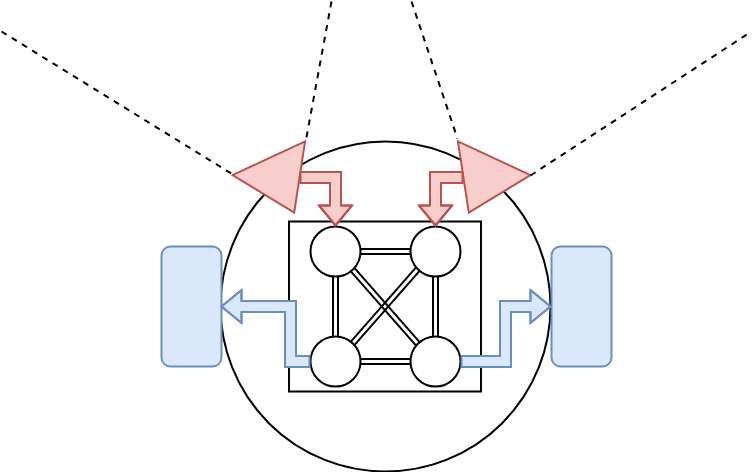
\includegraphics[width=0.9\textwidth,height=.35\textheight]{Imagenes/AgentSchema}
    \end{column}
\end{columns}
\end{block}
\end{frame}

\begin{frame}{Modelo}
  \begin{block}{Controlador basado en una CTRNN}
    \begin{equation*}
    	\dot{y_{i}}= \frac{1}{\tau_{i}} * \left ( -y_{i}+\sum_{j=1}^{N}w_{ji}*\sigma \left ( y_{j} + \theta _{j} \right ) + I_{i} \right ) \qquad i =1,2,...,N
    \end{equation*}
    \begin{columns}
      \begin{column}{0.47\textwidth}
          \begin{itemize}
            \item $\dot{y_{i}}$: nueva activación (estado) de la neurona i.
            \item $\tau_{i}$: constante de tiempo de la neurona i.
            \item $y_{i}$: activación actual de la neurona i.
            \item $w_{ji}$: peso de la conexión entre las neuronas i y j.
          \end{itemize}
      \end{column}
      \begin{column}{0.5\textwidth}
        \begin{itemize}
          \item $\sigma ()$: función sigmoide de activación.
          \item $y_{i}$: activación actual de la neurona j.
          \item $\theta_{j}$: bias de la neurona j.
          \item $I_{i}$: entrada de la neurona i.
        \end{itemize}
      \end{column}
    \end{columns}
  \end{block}
\end{frame}

\begin{frame}{Modelo}
  \begin{columns}
    \begin{column}{0.47\textwidth}
      \begin{equation*}
        \sigma (x)=\frac{1}{1+e^{-x}}
      \end{equation*}
        \begin{itemize}
          \item Recordamos: $x = y_{j} + \theta_{j}$.
          \item Devuelve valores entre 0 y 1.
        \end{itemize}
    \end{column}
    \begin{column}{0.5\textwidth}
      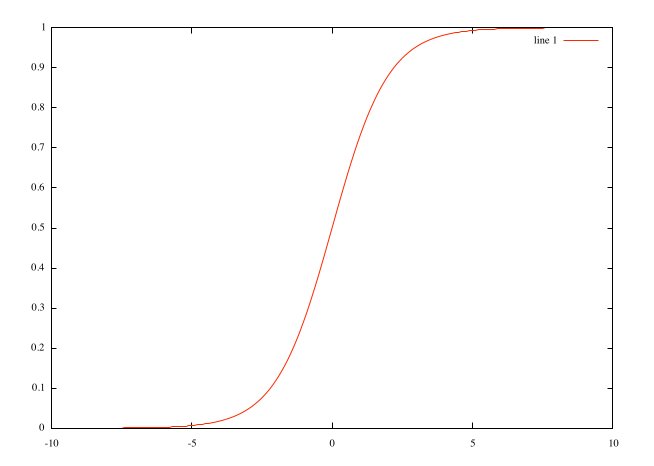
\includegraphics[width=1.0\textwidth,height=.50\textheight]{Imagenes/Sigmoid}
    \end{column}
  \end{columns}
  \begin{itemize}
    \item Se han seleccionado estas redes porque:
    \begin{itemize}
      \item Permiten simular cualquier sistema dinámico.
      \item Son las más fieles al funcionamiento biológico las activaciones neuronales.
    \end{itemize}
  \end{itemize}
\end{frame}

\begin{frame}{Modelo}
\begin{block}{Homeostasis}

\end{block}
\end{frame}

\begin{frame}{Modelo}
\begin{block}{Algoritmo genético}
  \begin{itemize}
    \item Utilizado para entrenar a los agentes (\textbf{Computación Evolutiva}).
    \item Agentes codificados como vector de reales y enteros.
  \end{itemize}
  \begin{figure}
    \centering
  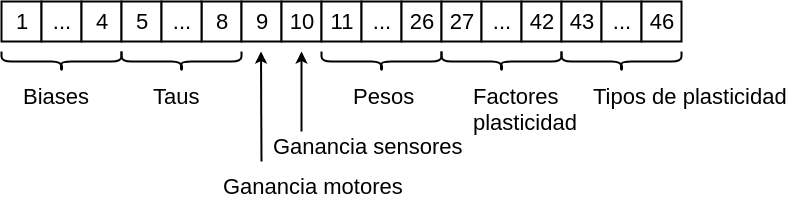
\includegraphics[width=0.7\textwidth,height=.3\textheight]{Imagenes/vector0}
\end{figure}
\end{block}
\end{frame}

\begin{frame}{Modelo}
Funcionamiento:
  \begin{enumerate}
    \item Generación de \textbf{población inicial} (primera generación).
    \item Evaluación de la generación mediante la \textbf{función fitness}.
    \item \textbf{Selección} de los mejores individuos de la generación.
    \item Creación de una nueva generación a partir de los individuos seleccionados (mediante \textbf{recombinaciones} y \textbf{mutaciones}).
    \item Volver al punto 2 hasta que el mejor individuo de la generación actual cumpla con las expectativas.
  \end{enumerate}
  Algunas anotaciones sobre el algoritmo genético:
  \begin{itemize}
    \item Población inicial de \textbf{60} candidatos.
    \item Función de selección de torneo.
    \item Función de recombinación uniforme.
    \item Función de mutación básica.
  \end{itemize}
\end{frame}

\section{Agente individual}
\subsection{Controlador}
\begin{frame}{Agente individual: Controlador}
  \begin{itemize}
    \item Agente con capacidades de fototaxis individual y plasticidad.
    \item Dos sensores luminosos y dos motores.
    \item Simetría en las ganancias de los motores y de los sensores.
    \item Finalidad: comprobar el correcto funcionamiento de la implementación de la fototaxis y la plasticidad.
  \end{itemize}
  \begin{figure}
    \centering
  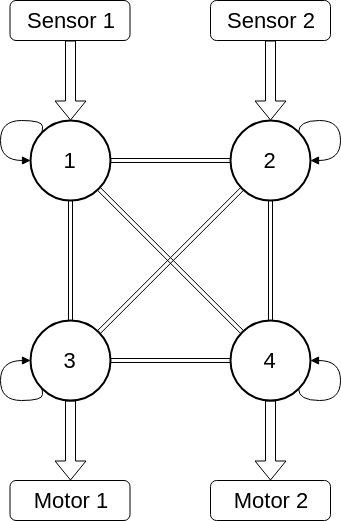
\includegraphics[width=0.25\textwidth,height=0.5\textheight]{Imagenes/Agent0Controller}
\end{figure}
\end{frame}

\subsection{Función fitness}
\begin{frame}{Agente individual: Función fitness}
  \begin{itemize}
    \item Un agente de tipo 0 situado en (0,0).
    \item De forma progresiva aparecen 6 luces a una distancia determinada del agente.
    \item Cada luz está encendida un número de ciclos aleatorio (dentro de un rango).
    \item Solamente una luz encendida al mismo tiempo.
    \item Se busca recompensar:
    \begin{itemize}
      \item Que para cada luz, el agente acabe más cerca de la luz que cuando se encendió.
      \item Que para cada luz, el agente permanezca alrededor de ella el mayor número de ciclos posibles.
      \item Que para cada luz, el máximo número de neuronas del agente se mantengan estables.
    \end{itemize}
  \end{itemize}
\end{frame}

\begin{frame}{Agente individual: Función fitness}
\begin{itemize}
  \item Máxima fitness alcanzada: \textbf{0.81}.
\end{itemize}

\begin{equation*}
 \centering
  fitness = (0.34Fd + 0.54Fp + 0.12Fh)
\end{equation*}
\noindent\rule{14cm}{0.4pt}
\begin{equation*}
  Fd=\begin{cases}
0.0 & \text{ IF }\quad D_{f} > D_{i}  \\
1 - (D_{f} / D_{i}) & \text{ IF }\quad D_{f} \leq D_{i} \\
\end{cases}
\end{equation*}
\noindent\rule{14cm}{0.4pt}
\begin{equation*}
\centering
Fp = \frac{\text{Nº ciclos cerca de la luz}}{\text{Nº de ciclos que la luz ha estado encendida}}
\end{equation*}
\noindent\rule{14cm}{0.4pt}

\begin{equation*}
\centering
Fh = \frac{\text{Nº neuronas que no han perdido estabilidad}}{\text{Nº de neuronas del agente}}
\end{equation*}
\end{frame}

\subsection{Experimentos}
\begin{frame}{Agente individual: Experimentos}
  \begin{figure}
    \centering
  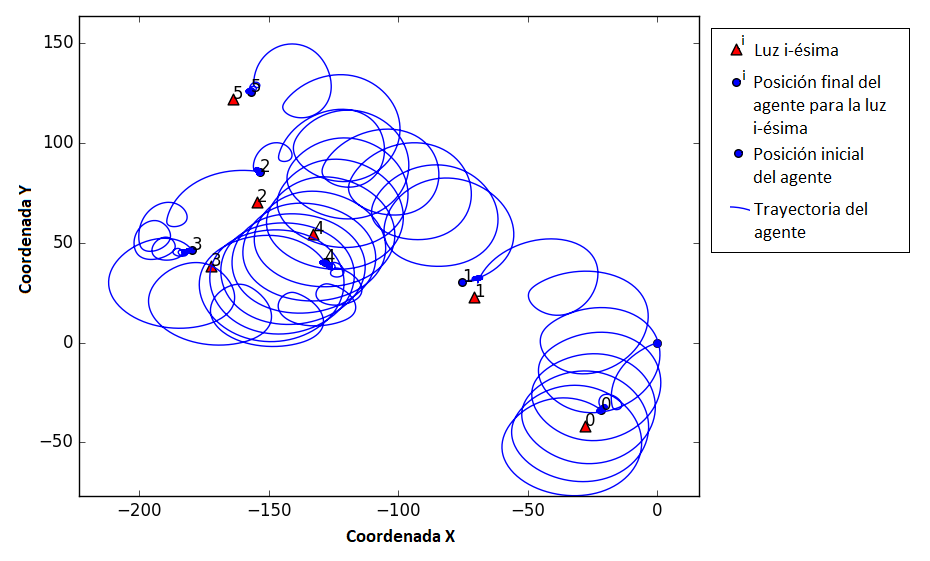
\includegraphics[width=0.7\textwidth,height=0.7\textheight]{Imagenes/Agente0Trayectoria}
\end{figure}
\end{frame}

\section{Agentes colectivos}
\begin{frame}{Agentes colectivos}
  \begin{itemize}
    \item Agentes con capacidades de fototaxis colectiva y plasticidad.
    \item Restricción colectiva: no más de \textbf{3} agentes pueden estar situados cerca de una luz al mismo tiempo.
    \item Dos sensores luminosos, dos sensores de agentes y dos motores.
    \item Simetría en las ganancias de los motores y de los sensores.
    \item Agente de tipo 1 (\textbf{aditivo}) $|$ Agente de tipo 2 (\textbf{estructural}).
    \item Un grupo de 5 agentes de tipo 1 y un grupo de 5 agentes de tipo 2.
  \end{itemize}
\end{frame}

\subsection{Controladores}
\begin{frame}{Agentes colectivos: Controladores}
  \begin{columns}
    \begin{column}{0.5\textwidth}
      \begin{block}{Agente 1 (aditivo)}
        \vspace{0.5cm}
      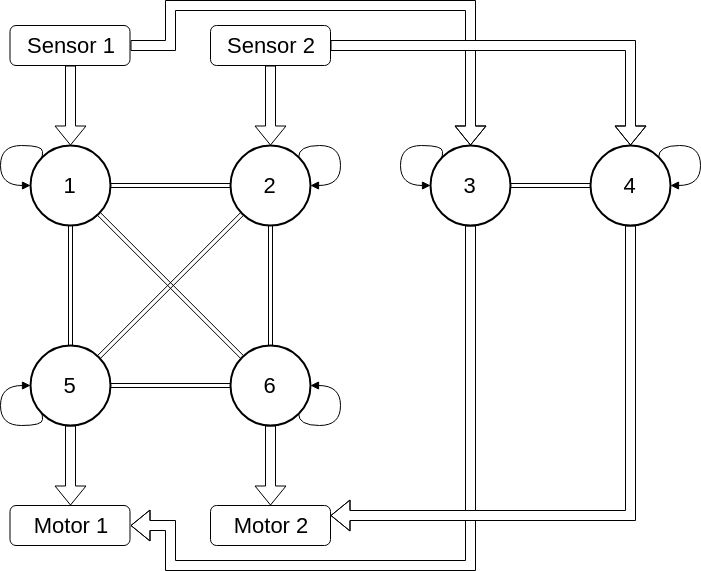
\includegraphics[width=0.8\textwidth,height=.50\textheight]{Imagenes/Agent1Controller}
    \end{block}
    \end{column}
    \begin{column}{0.5\textwidth}
      \begin{block}{Agente 2 (estructural)}
        \vspace{0.5cm}
      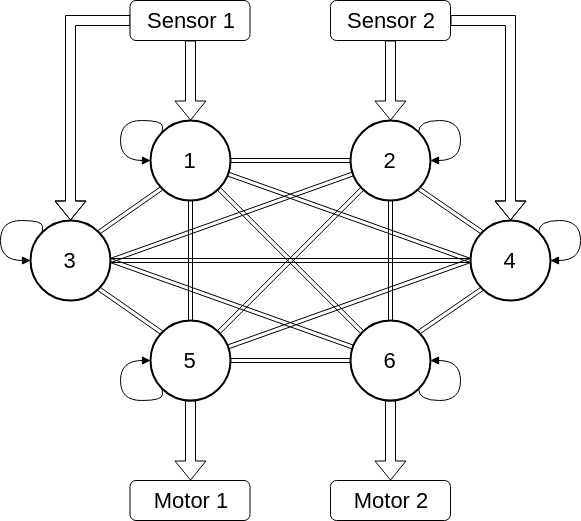
\includegraphics[width=0.8\textwidth,height=.50\textheight]{Imagenes/Agent2Controller}
      \end{block}
    \end{column}
  \end{columns}
\end{frame}

\subsection{Función fitness}
\begin{frame}{Agentes colectivos: Función fitness}
  \begin{itemize}
    \item Un grupo de 5 agentes de tipo 1 o tipo 2 situado en torno al (0,0).
    \item De forma progresiva aparecen 6 luces a una distancia mínima del centroide de los agentes.
    \item Cada luz está encendida un número de ciclos aleatorio (dentro de unos rangos).
    \item Solamente una luz encendida al mismo tiempo.
    \item Se busca recompensar:
    \begin{itemize}
      \item Que para cada luz, los agentes acaben más cerca de ella que cuando se encenció.
      \item Que para cada luz, se respete correctamente la restricción colectiva añadida.
      \item Que para cada luz, cada agente mantenga estables el mayor número posible de neuronas.
    \end{itemize}
  \end{itemize}

\end{frame}

\begin{frame}{Agentes colectivos: Función fitness}
  \begin{columns}
      \begin{column}{0.5\textwidth}
        \begin{block}{Agente 1 (aditivo)}
          \begin{itemize}
            \item Máxima fitness alcanzada: \textbf{0.472}.
          \end{itemize}
      \end{block}
      \end{column}
      \begin{column}{0.5\textwidth}
        \begin{block}{Agente 2 (estructural)}
          \begin{itemize}
            \item Máxima fitness alcanzada: \textbf{0.591}.
          \end{itemize}
        \end{block}
      \end{column}
  \end{columns}
  \begin{equation*}
   \centering
  	fitness = (0.44Fd + 0.44Fp + 0.12Fh)
  \end{equation*}
  \noindent\rule{14cm}{0.4pt}
  \begin{equation*}
    Fd = \frac{\sum_{k=1}^{5}(\frac{\sum_{j=1}^{NºLuces}Fd_{kj}}{NºLuces})}{5} \qquad \Rightarrow \qquad Fd_{kj}=\begin{cases}
    0.0 & \text{ IF }\quad D_{fkj} > D_{ikj}  \\
    1 - (D_{fkj} / D_{ikj}) & \text{ IF }\quad D_{fkj} \leq D_{ikj} \\
    \end{cases}
  \end{equation*}
  \noindent\rule{14cm}{0.4pt}
  \begin{equation*}
   \centering
  		Fp = \frac{\sum_{i= 1}^{\text{NºLuces}}\text{Contador}_{i}}{(\sum_{i =1}^{\text{NºLuces}}\text{Ciclos encendida}_{i}) * 3}
  \end{equation*}
  \noindent\rule{14cm}{0.4pt}
  \begin{equation*}
   \centering
  		Fh = \frac{\sum_{i = 1}^{Nº Luces}\frac{\sum_{k=1}^{5}(\frac{\text{Nº neuronas que no han perdido estabilidad}_{ki}}{\text{Nº de neuronas del agente}_{ki}})}{5}}{Nº Luces}
  \end{equation*}
\end{frame}

\subsection{Experimentos}
\begin{frame}{Agentes colectivos: Experimentos}
\begin{itemize}
  \item Se ha buscado comparar a los dos grupos de agentes respecto a:
  \begin{itemize}
    \item Sus trayectorias y el cumplimiento de la fototaxis colectiva.
    \item Las activaciones de sus neuronas.
    \item La robustez de los agentes ante ruido en los sensores.
    \item La robustez de los agentes ante ruido en la plasticidad.
  \end{itemize}
\end{itemize}
\end{frame}

\begin{frame}{Agentes colectivos: Experimentos (Trayectorias)}
  \begin{columns}
    \begin{column}{0.50\textwidth}
      \begin{block}{Agente 1 (aditivo)}
        \vspace{0.5cm}
      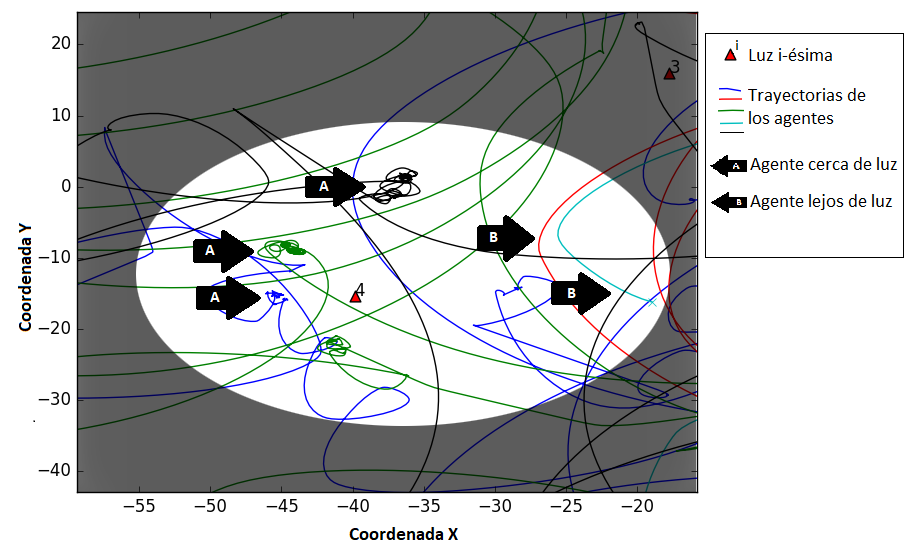
\includegraphics[width=1.1\textwidth,height=.6\textheight]{Imagenes/Agente1Trayectoria}
    \end{block}
    \end{column}
    \begin{column}{0.5\textwidth}
      \begin{block}{Agente 2 (estructural)}
        \vspace{0.5cm}
      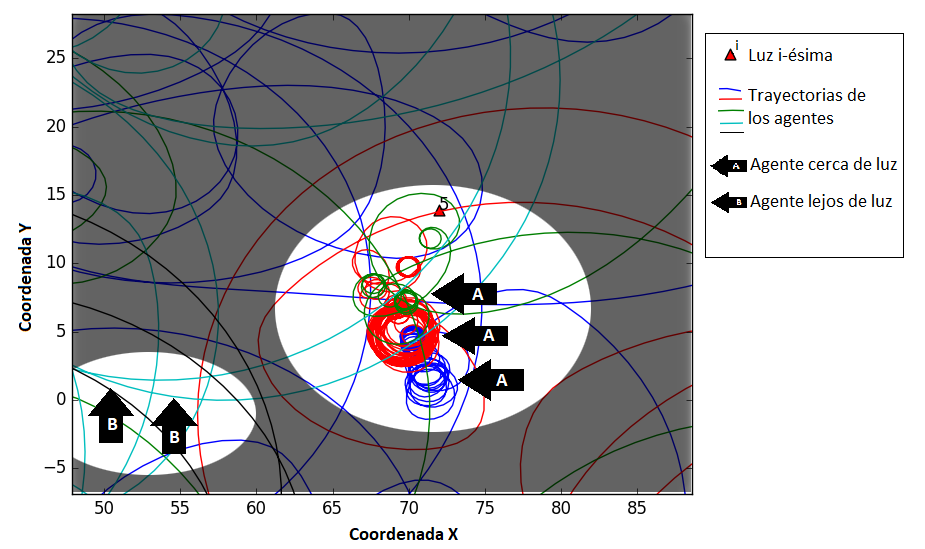
\includegraphics[width=1.1\textwidth,height=.6\textheight]{Imagenes/Agente2Trayectoria}
      \end{block}
    \end{column}
  \end{columns}
\end{frame}

\begin{frame}{Agentes colectivos: Experimentos (Activaciones neuronales)}
  \begin{columns}
    \begin{column}{0.47\textwidth}
      \begin{block}{Agente 1 (aditivo)}
        \vspace{0.5cm}
      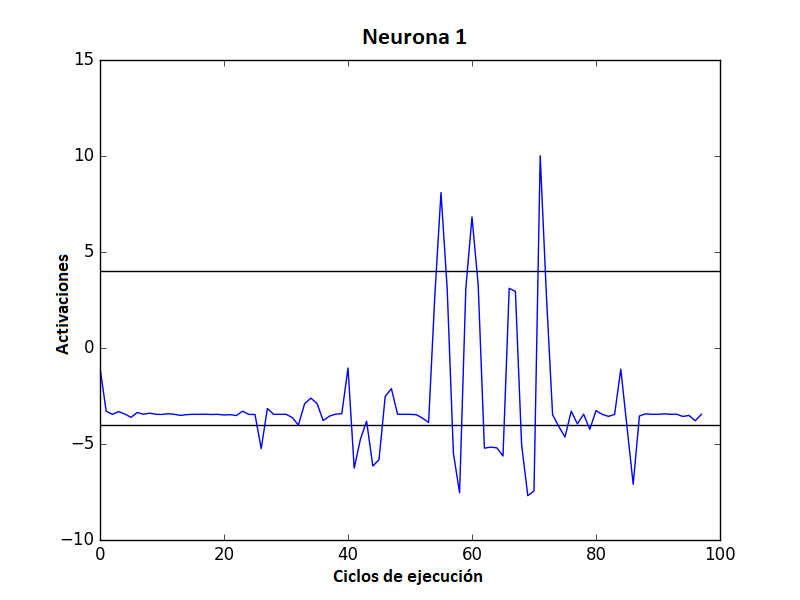
\includegraphics[width=1.0\textwidth,height=.6\textheight]{Imagenes/Neurona0}
    \end{block}
    \end{column}
    \begin{column}{0.5\textwidth}
      \begin{block}{Agente 2 (estructural)}
        \vspace{0.5cm}
      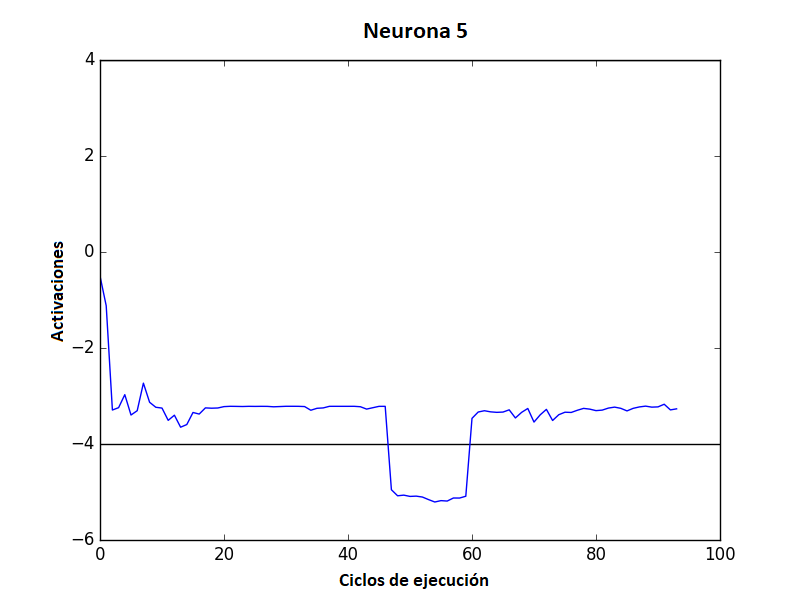
\includegraphics[width=1.0\textwidth,height=.6\textheight]{Imagenes/Neurona4}
      \end{block}
    \end{column}
  \end{columns}
\end{frame}

\begin{frame}{Agentes colectivos: Experimentos (Robustez en los sensores)}
  \begin{itemize}
    \item Comprobar si la fitness se ve afectada por el ruido en los sensores.
    \item Para cada grupo, \textbf{30} mediciones de la fitness para cada nivel de ruido.
    \item Factores de ruido probados: 0.0, 0.2, 0.34 y 0.44.
  \end{itemize}
  \vspace{-0.5cm}
  \begin{columns}
    \begin{column}{0.47\textwidth}
      \begin{block}{Agente 1 (aditivo)}
      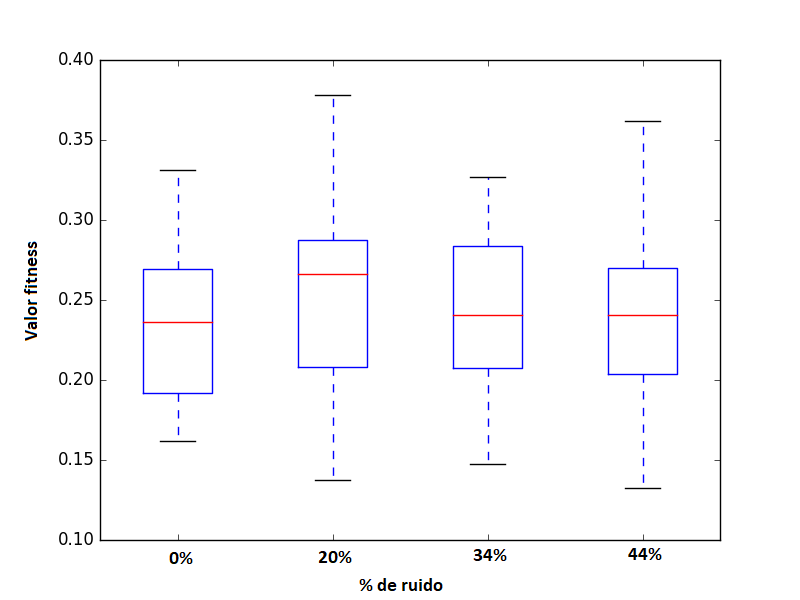
\includegraphics[width=1.0\textwidth,height=.6\textheight]{Imagenes/BoxPlot1}
    \end{block}
    \end{column}
    \begin{column}{0.5\textwidth}
      \begin{block}{Agente 2 (estructural)}
      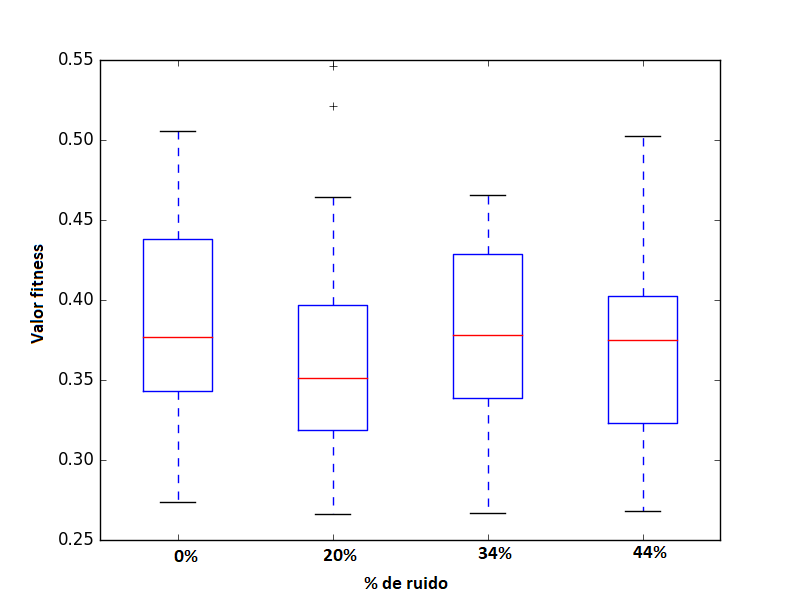
\includegraphics[width=1.0\textwidth,height=.6\textheight]{Imagenes/BoxPlot2}
      \end{block}
    \end{column}
  \end{columns}
\end{frame}

\begin{frame}{Agentes colectivos: Experimentos (Robustez en los sensores)}
  \begin{columns}
    \begin{column}{0.47\textwidth}
      \begin{block}{Agente 1 (aditivo)}

    \end{block}
    \end{column}
    \begin{column}{0.5\textwidth}
      \begin{block}{Agente 2 (estructural)}

      \end{block}
    \end{column}
  \end{columns}
\end{frame}


\begin{frame}{Agentes colectivos: Experimentos}
\begin{block}{Robustez en la plasticidad}

\end{block}
\end{frame}



% \subsection{Función fitness}
% \begin{frame}{Agentes colectivos: Función fitness}
%   \begin{columns}
%     \begin{column}{0.47\textwidth}
%       \begin{block}{Agente 1 (aditivo)}
%         \vspace{0.5cm}
%       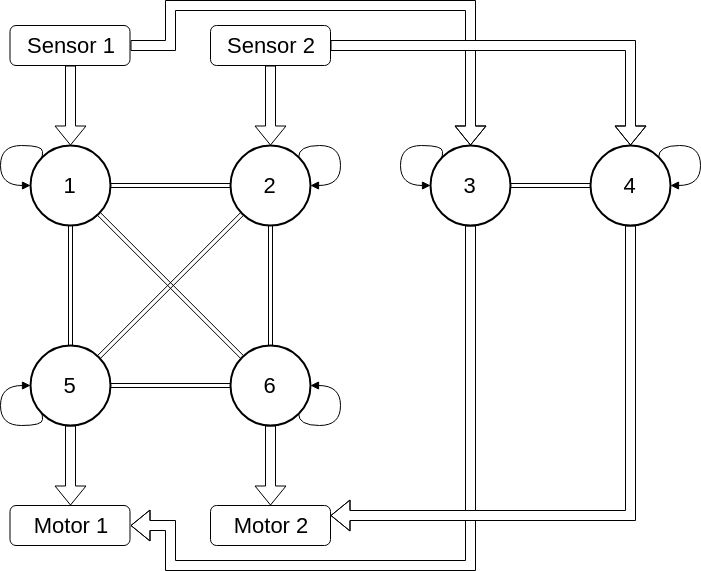
\includegraphics[width=0.8\textwidth,height=.50\textheight]{Imagenes/Agent1Controller}
%     \end{block}
%     \end{column}
%     \begin{column}{0.5\textwidth}
%       \begin{block}{Agente 2 (estructural)}
%         \vspace{0.5cm}
%       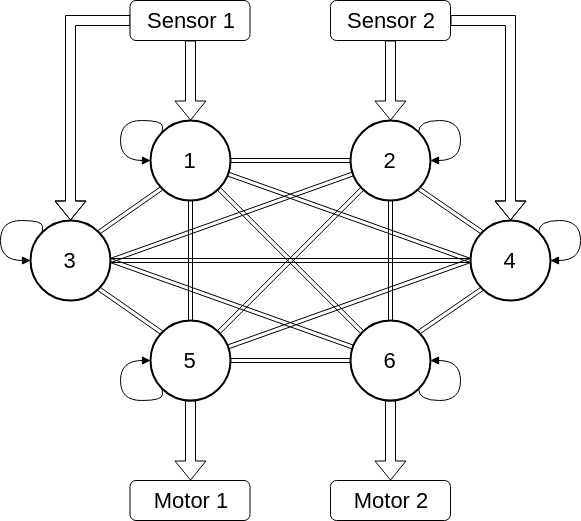
\includegraphics[width=0.8\textwidth,height=.50\textheight]{Imagenes/Agent2Controller}
%       \end{block}
%     \end{column}
%   \end{columns}
% \end{frame}


\end{document}
